\chapter{Fundamentação Teórica}
    \label{fundamentacao_teorica}
    
    Este capítulo apresenta a fundamentação teórica necessária para a compreensão dos conceitos e técnicas empregados neste trabalho, fornecendo o embasamento conceitual que sustenta as escolhas metodológicas adotadas posteriormente. O foco recai sobre o controle de enxames de veículos aéreos não tripulados por meio de aprendizado por reforço multiagente, bem como sobre a utilização de máquinas de recompensa para a modelagem de tarefas complexas.

    Inicialmente, são abordados os fundamentos dos sistemas de veículos aéreos não tripulados, contemplando seus principais componentes, modelos dinâmicos e sistemas de controle de voo, de modo a contextualizar as limitações físicas e operacionais consideradas nas simulações. Em seguida, são introduzidos os conceitos relacionados a enxames de VANTs, incluindo arquiteturas de coordenação, comportamentos coletivos e os principais desafios associados ao controle distribuído desses sistemas.

    Na sequência, são apresentados os fundamentos do aprendizado por reforço, estabelecendo a base conceitual necessária para a compreensão do aprendizado por reforço multiagente. Posteriormente, são discutidas as particularidades desse paradigma, com ênfase nas abordagens algorítmicas adotadas na literatura e no algoritmo Multi-Agent Proximal Policy Optimization.

    Por fim, o capítulo introduz as máquinas de recompensa como um formalismo para a especificação estruturada de objetivos e tarefas sequenciais, destacando sua integração com métodos de aprendizado por reforço e sua relevância para cenários multiagentes complexos.


    \section{Sistemas de Veículos Aéreos Não Tripulados}

    Esta seção fornece uma visão geral dos conceitos fundamentais necessários para compreender os sistemas de VANT, seus mecanismos de controle e os princípios de coordenação em enxames. Começamos detalhando os principais componentes e classificações dos VANTs, seguido por uma discussão sobre estratégias de controle e, por fim, as arquiteturas de enxames.

    \subsection{Principais componentes de um VANT}
        Um VANT (Veículo Aéreo Não Tripulado) consiste em diversos componentes essenciais que possibilitam sua operação autônoma. Estes incluem:
        \begin{itemize}
            \item \textbf{Estrutura do Drone:} O quadro (ou frame) de um drone é a estrutura física que serve como base para todos os seus componentes. Ele é responsável por suportar os motores, hélices, controladores de voo, baterias, sensores e demais módulos eletrônicos. Em geral, o frame é projetado para ser leve, rígido e resistente, a fim de garantir estabilidade e eficiência durante o voo.
            \item \textbf{Sistema de Propulsão:} Motores elétricos e hélices para UAVs de múltiplos rotores ou motores a combustão para drones de asa fixa de maior porte.
            \item \textbf{Controladora de Voo:}  É o componente central do drone responsável por interpretar os dados dos sensores (como giroscópios, acelerômetros, GPS e magnetômetros) e enviar comandos precisos aos motores para estabilizar e controlar o voo.
            \item \textbf{Computador embarcado:} Sistema de computação embarcada que realiza o processamento de dados oriundos dos sensores, do controlador de voô e da estação solo. Geralmente neste componente que ocorre a execução dos algoritmos de visão computacional essenciais para a navegação do drone. Neste componente que as decisões de alto nível são tomadas e repassadas à controladora de voo.
            \item \textbf{Sensores:} Unidades de Medição Inercial (IMU), GPS, LiDAR, câmeras e barômetros, que auxiliam na navegação, estabilidade e percepção do ambiente.
            \item \textbf{Sistema de Comunicação:} Links de dados para telemetria, controle e coordenação entre os agentes.
        \end{itemize}

        % Os UAVs podem ser classificados com base em:
        % \begin{enumerate}
        %     \item \textbf{Tamanho e Peso:} UAVs nano, micro, pequenos, médios e grandes.
        %     \item \textbf{Nível de Autonomia:} Drones pilotados remotamente, semiautônomos e totalmente autônomos.
        %     \item \textbf{Capacidades de Voo:} UAVs de asa fixa (maior autonomia), UAVs de rotores (capacidade de pairar) e UAVs híbridos.
        % \end{enumerate}

        %\noindent\textbf{TO-DO:} Criar Diagrama ilustrando os componentes que constituem um VANT, ou tirar foto do drone no Laboratorio

    \subsection{Dinâmica de Voo de um Quadricóptero}

        Neste trabalho, adota-se como plataforma aérea um veículo multirrotor com quatro motores, denominado quadricóptero (\textit{quadcopter}). Esse tipo de VANT apresenta seis graus de liberdade, sendo três translacionais e três rotacionais, associados aos movimentos de rolagem (\textit{roll}), arfagem (\textit{pitch}) e guinada (\textit{yaw}). A modelagem de sua dinâmica é fundamental para compreender a relação entre os comandos aplicados aos rotores e o movimento resultante do veículo.

        Considere o vetor $\boldsymbol{\omega} = [\omega_1, \omega_2, \omega_3, \omega_4]$, que representa as velocidades angulares dos quatro motores, e o vetor de ângulos de Euler $[\phi, \theta, \psi]$, correspondente à orientação do veículo no espaço. As forças e momentos gerados pelos rotores podem ser expressos pelas seguintes relações:

        \begin{align}
            u_f &= b(\omega_1^2 + \omega_2^2 + \omega_3^2 + \omega_4^2), \quad \text{[Empuxo total]},\\
            u_\phi &= bL(\omega_4^2 - \omega_2^2), \quad \text{[Momento de rolagem]}, \\
            u_\theta &= bL(\omega_3^2 - \omega_1^2), \quad \text{[Momento de arfagem]}, \\
            u_\psi &= d(\omega_1^2 - \omega_2^2 + \omega_3^2 - \omega_4^2), \quad \text{[Momento de guinada]},\\
            m\ddot{\mathbf{p}} &= -m\mathbf{g} + \mathbf{R}\,\mathbf{e}_3\,u_f, \quad \text{[Dinâmica translacional]}.
        \end{align}

        Nessas equações, $b$ representa o coeficiente de empuxo dos rotores, $d$ o coeficiente de arrasto aerodinâmico, $L$ a distância entre cada motor e o centro de massa do veículo, $\mathbf{R}$ a matriz de rotação do referencial do corpo para o referencial inercial, $\mathbf{e}_3 = [0,0,1]^\top$ o eixo $z$ do corpo, $m$ a massa total do VANT e $\mathbf{g}$ o vetor de aceleração gravitacional. Os sinais associados aos momentos dependem da convenção adotada para a numeração e o sentido de rotação dos motores.

        A dinâmica rotacional do quadricóptero pode ser descrita de forma compacta por:

        \begin{equation}
            \mathbf{I}\dot{\boldsymbol{\Omega}} + \boldsymbol{\Omega} \times (\mathbf{I}\boldsymbol{\Omega}) = \boldsymbol{\tau},
        \end{equation}

        em que $\boldsymbol{\Omega}$ representa o vetor de velocidades angulares do corpo, $\mathbf{I}$ a matriz de inércia e $\boldsymbol{\tau} = [u_\phi, u_\theta, u_\psi]^\top$ o vetor de momentos aplicados.

        A partir desse modelo, observa-se que o movimento do quadricóptero é obtido por meio da coordenação adequada das velocidades angulares dos rotores, permitindo a geração controlada de forças e momentos responsáveis tanto pela translação quanto pela orientação do veículo. Dessa forma, o sistema de controle de voo deve atuar diretamente sobre $\boldsymbol{\omega}$, de modo a garantir que a dinâmica resultante siga a trajetória e a atitude desejadas.

        \begin{figure}[H]
            \centering
            \includegraphics[scale=0.5]{fig/uav_dynamics_3.png}   
            \caption{Diagrama esquemático da dinâmica de um VANT com quatro motores.}
            \label{fig:dynamic_quadrotor}
        \end{figure}

    \subsection{Sistemas de Controle de Voo}
        %TODO verificar referencias e equacoes da dinamica do quadricoptero
        Um sistema de controle de voo de UAV é o mecanismo central que mantém e ajusta a orientação de um drone durante o voo, gerenciando o yaw, pitch e roll. Esse sistema de controle depende do feedback dos sensores para comparar continuamente a atitude real com o estado desejado, efetuando correções rápidas para garantir a estabilidade. Dentre as principais estratégias existente para o controle de voo, existem desde técnicas clássicas até métodos avançados baseados em IA. 

    \subsubsection*{\textbf{Controle Clássico Baseado em PID}}
        Os controladores PID nos sistemas de voo utilizam da teoria clássica de controle, especialmente na análise no domínio da frequência das funções de transferência. Ao representar o comportamento dinâmico do UAV por meio de uma função de transferência, é possível estudar como o sistema responde a diferentes frequências. O controlador PID ajusta os ganhos proporcional, integral e derivativo para modelar a resposta em frequência, aprimorando a estabilidade e o desempenho do sistema. Esse processo de ajuste garante que a atitude do drone — seu roll, pitch e yaw — permaneça responsiva aos comandos de controle, minimizando ultrapassagens e oscilações. Em essência, o projeto do controlador PID aproveita os insights matemáticos obtidos a partir da resposta em frequência do sistema, possibilitando uma estratégia de controle precisa e robusta para manter um desempenho de voo ideal.
        O sinal de controle de saída é matematicamente definido no domínio do tempo como:
        \begin{equation}
            u(t) = K_p \, e(t) + K_i \int_0^t e(\tau) \, d\tau + K_d \, \frac{d}{dt} e(t).
        \end{equation}
        onde:
        \begin{itemize}
            \item $u(t)$ é o comando de controle enviado aos atuadores.
            \item $e(t)$ é o erro entre o estado desejado e o real.
            \item $K_p$, $K_i$ e $K_d$ são os ganhos proporcional, integral e derivativo, respectivamente.
        \end{itemize}
        Aplicando a transformada de Laplace o sinal de controle torna-se:
        \begin{equation}
            C(s) = K_p + \frac{K_i}{s} + K_d s.
        \end{equation}
        \begin{figure}[H]
            \centering
        \begin{center}
        \begin{tikzpicture}[auto, node distance=1cm]

            % Nodes
            \node [sum] (sum) {$+$};
        \node [block, right=of sum] (controller) {$C(s) = K_p + \frac{K_i}{s} + K_d s$};
            \node [block, right=of controller] (quad) {$G(s) = \frac{1}{I s^2}$};
            \node [coordinate, right=of quad] (output) {};
            \node [coordinate, below=1.5cm of quad] (feedback) {};
            \node [coordinate, left=of sum] (input) {};

            % Arrows
            \draw [arrow] (input) -- node{\Large$R(s)$} (sum);
            \draw [arrow] (sum) -- (controller);
            \draw [arrow] (controller) -- node{\Large$u(t)$} (quad);
            \draw [arrow] (quad) -- node{\Large$Y(s)$} (output);
            \draw [arrow] (output) |- (feedback) -| node[pos=0.9, above]{\Large$-$} (sum);

        \end{tikzpicture}
        \end{center}
            \caption{Malha de controle fechada quadrotor.}
            \fonte{Elaborado pelo autor.}
            \label{fig:malha_fechada_drone}
        \end{figure}
        Em que $G(s)$ representa a função transferência de malha aberta que modela a dinâmica do drone com 4 rotores, sendo $I$  momento de inércia sob os respectivos eixos. $R(s)$ indica a entrada de referência, ou seja, os ângulos roll, pitch e yaw desejados. $Y(s)$ representa a saída obtida a partir dos sensores IMU do drone, que são retroalimentados para computação do erro, ajustando a entrada do controlador.

        %\noindent\textbf{Sugestão de Ilustração:} Diagrama em blocos de um sistema de controle de voo de UAV usando PID, mostrando comandos de entrada, loops de feedback e resposta dos atuadores.


        
%%%%%% ######## Enxame de VANTs ########%%%%%%
    
\section{Enxames de Veículos Aéreos Não Tripulados}
    \subsection{Definição }
        Um \textbf{enxame de veículos aéreos não tripulados (VANTs)} refere-se a um conjunto de drones autônomos ou semiautônomos que operam de forma cooperativa e distribuída com o objetivo de cumprir uma missão comum. Esse paradigma é fortemente inspirado em comportamentos coletivos observados na natureza, como colônias de insetos sociais, e caracteriza-se por propriedades como robustez, flexibilidade e eficiência operacional. Estudos clássicos, como os de \citeonline{brambilla2013swarm} e \citeonline{chung2018survey}, consolidaram esse conceito no contexto da robótica móvel e aérea.

        Entre as principais propriedades que caracterizam um enxame de VANTs, destacam-se:
        \begin{itemize}
            \item \textbf{Arquitetura}: define a forma como as decisões são tomadas e distribuídas entre os agentes, podendo assumir configurações centralizadas, descentralizadas ou híbridas, conforme a taxonomia apresentada por \citeonline{bayndir2016review}.
            \item \textbf{Escalabilidade}: capacidade do sistema de manter desempenho adequado à medida que o número de agentes aumenta, aspecto fundamental para operações com dezenas ou centenas de VANTs \cite{chung2018survey}.
            \item \textbf{Adaptabilidade}: habilidade do enxame de reagir a mudanças no ambiente, como obstáculos, alvos móveis ou novas missões, sendo essencial em cenários dinâmicos e não estruturados, conforme discutido por \citeonline{ollero2021past}.
            \item \textbf{Redundância}: tolerância a falhas obtida pela distribuição de funções entre múltiplos agentes, permitindo a continuidade da missão mesmo diante da perda de um ou mais VANTs.
        \end{itemize}

    \subsection{Arquiteturas de Enxames}

        As arquiteturas de controle de enxames de VANTs podem ser classificadas em três categorias principais: centralizada, descentralizada e híbrida, de acordo com o grau de distribuição do processo decisório.

        Na \textbf{arquitetura centralizada} (Figura~\ref{fig:arquitetura_central}), um nó controlador central, geralmente representado por uma estação solo, é responsável por coletar informações dos VANTs e emitir comandos de controle. Essa abordagem facilita a coordenação global e possibilita a execução de otimizações centralizadas. Contudo, apresenta limitações significativas, como baixa escalabilidade e a presença de um ponto único de falha, tornando-se inadequada para missões em larga escala ou ambientes com conectividade instável.

        A \textbf{arquitetura descentralizada} (Figura~\ref{fig:arquitetura_desc}) distribui a tomada de decisão entre os próprios VANTs, que atuam com base em observações locais e comunicação entre pares. Nessa configuração, cada agente deve possuir maior autonomia, frequentemente viabilizada por algoritmos de inteligência artificial. Essa abordagem apresenta elevada robustez e escalabilidade, porém impõe desafios adicionais de coordenação e pode resultar em soluções subótimas quando comparada a abordagens centralizadas.

        Por fim, a \textbf{arquitetura híbrida} (Figura~\ref{fig:arquitetura_hibrida}) combina elementos das duas abordagens anteriores. Um componente central é responsável pelo planejamento de alto nível, como a atribuição de tarefas, enquanto a execução ocorre de forma descentralizada entre os VANTs. Essa configuração busca equilibrar controle global e autonomia local, oferecendo maior flexibilidade e resiliência operacional.

        \begin{figure}[h]
            \centering
            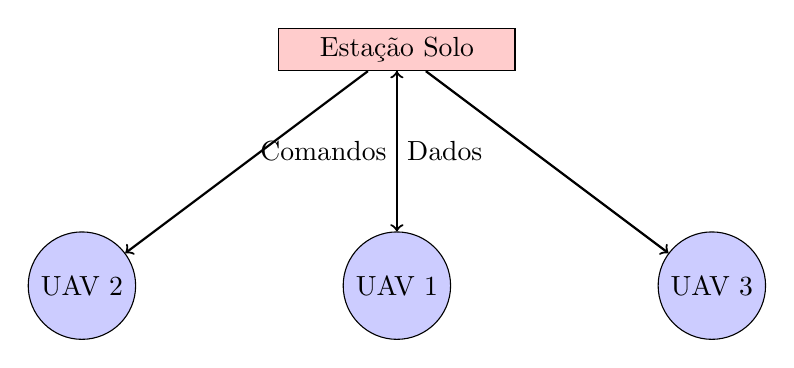
\begin{tikzpicture}[node distance=2cm]
            % Controlador Central
            \node[draw, rectangle, fill=red!20, minimum width=3cm] (central) {Estação Solo};
            % UAVs
            \node[draw, circle, fill=blue!20, below of=central, yshift=-1cm] (uav1) {UAV 1};  
            \node[draw, circle, fill=blue!20, left of=uav1, xshift=-2cm] (uav2) {UAV 2};  
            \node[draw, circle, fill=blue!20, right of=uav1, xshift=2cm] (uav3) {UAV 3};  
            % Conexões
            \draw[->, thick] (central) -- (uav1) node[midway, left] {Comandos};  
            \draw[->, thick] (central) -- (uav2);  
            \draw[->, thick] (central) -- (uav3);  
            \draw[->, thick, dashed] (uav1) -- (central) node[midway, right] {Dados};  
        \end{tikzpicture}
            \caption{Arquitetura Centralizada.}
            \fonte{Elaborado pelo autor.}
            \label{fig:arquitetura_central}
        \end{figure}

        \begin{figure}[h]
            \centering
            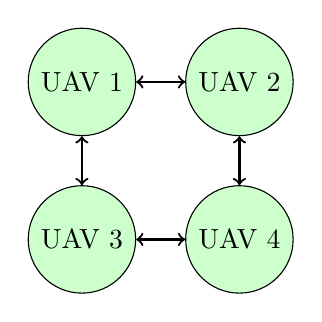
\begin{tikzpicture}[node distance=2cm]
            % UAVs
            \node[draw, circle, fill=green!20] (uav1) {UAV 1};  
            \node[draw, circle, fill=green!20, right of=uav1] (uav2) {UAV 2};  
            \node[draw, circle, fill=green!20, below of=uav1] (uav3) {UAV 3};  
            \node[draw, circle, fill=green!20, below of=uav2] (uav4) {UAV 4};  
            
            % Conexões peer-to-peer
            \draw[<->, thick] (uav1) -- (uav2);  
            \draw[<->, thick] (uav1) -- (uav3);  
            \draw[<->, thick] (uav2) -- (uav4);  
            \draw[<->, thick] (uav3) -- (uav4);  
        \end{tikzpicture}
            \caption{Arquitetura Descentralizada.}
            \label{fig:arquitetura_desc}
        \end{figure}


        \begin{figure}[h]
            \centering
            \begin{tikzpicture}[node distance=3cm]
            % Central Planner
            \node[draw, rectangle, fill=orange!20] (central) {Estação Solo};
            % Subgroup Leaders
            \node[draw, diamond, fill=purple!20, below left of=central] (lider1) {Lider 1};  
            \node[draw, diamond, fill=purple!20, below right of=central] (lider2) {Lider 2};  
            % Planner connections
            \draw[->, dashed, thick] (central) -- (lider1);  
            \draw[->, dashed, thick] (central) -- (lider2);  
            % Subgroups
            \node[draw, circle, fill=cyan!20, below left of=lider1] (uav1) {UAV A};  
            \node[draw, circle, fill=cyan!20, right of=uav1] (uav2) {UAV B};
            \node[draw, circle, fill=cyan!20, right of=uav2] (uav3) {UAV C};  
            \node[draw, circle, fill=cyan!20, below right of=lider2] (uav4) {UAV D};  
            %\node[draw, circle, fill=cyan!20, left of=uav4] (uav5) {UAV E};  
            % Peer-to-peer connections
            \draw[<->, thick] (lider1) -- (uav1); 
            \draw[<->, thick] (lider1) -- (uav2);  
            \draw[<->, thick] (uav1) -- (uav2);  
            \draw[<->, thick] (lider2) -- (uav3);  
            \draw[<->, thick] (lider2) -- (uav4);
            \draw[<->, thick] (uav3) -- (uav4);
            \draw[<->, thick] (uav2) -- (uav3);  
        \end{tikzpicture}
            \caption{Arquitetura Híbrida.}
            \fonte{Elaborado pelo autor.}
            \label{fig:arquitetura_hibrida}
        \end{figure}


    \subsection{Aplicações e Comportamentos de Enxames de VANTs}

        Os enxames de VANTs têm sido amplamente explorados em diferentes domínios devido à sua capacidade de realizar missões cooperativas de forma eficiente e escalável. Entre as principais aplicações, destacam-se tarefas de vigilância e reconhecimento, como patrulhamento de fronteiras e rastreamento de alvos, nas quais múltiplos VANTs podem cobrir grandes áreas simultaneamente. Em cenários de resposta a desastres, esses sistemas são empregados em operações de busca e resgate e avaliação de danos, permitindo atuação segura em ambientes de difícil acesso.

        Na agricultura de precisão, enxames de VANTs são utilizados para monitoramento de culturas, detecção de pragas e pulverização seletiva, enquanto em contextos de comunicação podem atuar como redes móveis temporárias para fornecer conectividade em áreas remotas ou durante emergências. Em aplicações militares, esses sistemas são empregados em missões coordenadas de reconhecimento, guerra eletrônica e operações ofensivas, explorando sua adaptabilidade e redundância.

        A execução eficiente dessas aplicações depende de um conjunto de \textbf{comportamentos coletivos} característicos dos sistemas de enxame. Dentre eles, destacam-se a formação de voo, que permite a manutenção de padrões geométricos organizados; a alocação dinâmica de tarefas entre os agentes; o planejamento colaborativo de trajetórias e desvio de obstáculos; a tomada de decisão coletiva; e a autorreconfiguração do enxame diante de falhas ou perdas de agentes. Esses comportamentos emergem da interação local entre os VANTs e são fundamentais para a robustez e flexibilidade do sistema.


    
    \subsection{Principais Desafios no Controle de Enxames de VANTs}
        Apesar de suas vantagens, o controle de enxames de VANTs envolve diversos desafios técnicos e operacionais, especialmente em ambientes reais e dinâmicos. A Tabela~\ref{tab:desafios_enxame} sintetiza os principais desafios associados a esse problema.

        \begin{table}[H]
        \centering
        \caption{Principais desafios no controle de enxames de VANTs}
        \label{tab:desafios_enxame}
        \begin{tabular}{p{4cm} p{10cm}}
        \toprule
        \textbf{Desafio} & \textbf{Descrição} \\
        \midrule
        Não estacionariedade &
        A presença de múltiplos agentes aprendendo ou tomando decisões simultaneamente altera continuamente a dinâmica do ambiente percebido por cada VANT. \\

        Observabilidade parcial &
        Cada agente possui acesso limitado ao estado global do sistema, dificultando a coordenação e a tomada de decisões cooperativas. \\

        Escalabilidade &
        O aumento do número de VANTs eleva os custos computacionais e de comunicação, dificultando o controle eficiente do enxame. \\

        Ambientes dinâmicos &
        Mudanças no ambiente, obstáculos móveis e alvos dinâmicos exigem adaptação e replanejamento em tempo real. \\

        Restrições físicas &
        Limitações de autonomia energética, capacidade computacional embarcada e precisão de sensores e atuadores. \\

        Segurança e resiliência &
        Vulnerabilidade a falhas, interferências eletromagnéticas e ataques cibernéticos, além da presença de agentes adversários. \\
        \bottomrule
        \end{tabular}
        \end{table}

        Esses desafios evidenciam a necessidade de abordagens avançadas de controle e coordenação, motivando o uso de técnicas de aprendizado por reforço multiagente e arquiteturas distribuídas capazes de lidar com ambientes complexos, dinâmicos e parcialmente observáveis.

    
    % \section{Fundamentos do Aprendizado por Reforço}

    %     O Aprendizado por Reforço (Reinforcement Learning - RL) é um paradigma de aprendizado de máquina inspirado pela psicologia comportamental, onde um agente aprende a tomar decisões interagindo com um ambiente para maximizar recompensas cumulativas. Diferentemente do aprendizado supervisionado, no qual os modelos aprendem com dados rotulados, o RL depende de interações por tentativa e erro para descobrir estratégias ótimas. Segundo \citeonline{sutton2018reinforcement}, os conceitos fundamentais no RL são descritos como segue.
    %     \begin{figure}[!h]
    %         \centering
    %         \includegraphics[scale=0.6]{fig/rl_loop_uav.png}
    %         \caption{Exemplo de diagrama esquemático sistema RL com agente VANT.}
    %         \fonte{Autor.}
    %         \label{fig:rl_diagram}
    %     \end{figure}

    %     \subsection{Agente}
    %         O agente é o tomador de decisões dentro do framework de RL. Ele interage com o ambiente executando ações e aprende uma política (\textit{policy})—um mapeamento entre estados e ações que determina a tomada de decisões do agente. A política é o núcleo central do agente, de modo esta determina o comportamento do agente. Portanto a fase de treinamento do agente, consiste em encontrar uma política que maximize a recompensa acumulada (retorno) esperada ao longo do período de atuação do agente.
    %         A Figura \ref{fig:rl_diagram} ilustra o fluxo de interação entre o agente e o ambiente. 

    %     \subsection{Ambiente}
    %         O ambiente representa tudo fora do agente com o qual ele interage. Ele fornece ao agente um estado ou observação, que é uma representação da situação atual que o agente é capaz de perceber, e responde às ações do agente mudando para um novo estado e oferecendo feedback em forma de recompensa. 
    %         \begin{definition}[Framework RL]
    %         Formalmente, o framework de RL é modelado como um Processo de Decisão de Markov (MDP), definido pela tupla $\langle S,A,P,R \rangle$ onde:
    %         \begin{itemize}
    %             \item (\(S\)): Conjunto denominado espaço de estados. Neste trabalho o espaço de estados são o conjunto de observações que o drone obtém do ambiente. Informações como: pose do drone no espaço, pontos de nuvem das leituras do sensor LiDAR, imagens das câmeras do drone, GPS (latitude e longitude).
    %             \item (\(A\)): Conjunto denominado espaço de ações.
    %             \item \(P(s_{t+1}|s_t, a_t)\): Uma função de transição , que define a probabilidade de transição para o estado \(s_{t+1}\) ao realizar a ação \(a_t\) no estado \(s_t\).
    %             \item \(R(s, a)\): Função de recompensa, atribui um valor escalar ao estado observado pelo agente ao executar uma ação.
    %         \end{itemize}
                
    %         \end{definition}

    %     \subsection{Recompensa}
    %         A recompensa é um sinal de feedback escalar que quantifica o benefício imediato de uma ação tomada pelo agente. Este é o principal sinal que orienta o processo de aprendizado do agente. O objetivo do agente é maximizar a recompensa cumulativa (retorno) recebida ao longo do tempo. Isso envolve equilibrar recompensas imediatas e ganhos potenciais de longo prazo. O tipo de retorno mais utilizado é o \textbf{retorno esperado de horizonte infinito}, limitado o fator de desconto \(\gamma \in (0,1)\), definido como:
    %         \begin{equation}
    %             R(\tau) = \sum_{t=0}^{\infty} \gamma^{t}r_t.  
    %         \end{equation}
    %         onde $R(s_t, a_t)=r_t$ e $\tau=(s_0,a_0,s_1,a_1,...)$ representa um histórico de sequência de estados e ações tomadas no ambiente.

    %     \subsection{Política}
    %         A política (\(\pi\)) define o comportamento do agente. É uma função ou distribuição de probabilidade que mapeia estados para ações. Políticas podem ser determinísticas (\(a_t = \pi(s_t) \)) ou estocásticas \(\pi(a_t|s_t) \in [0,1]\).

    %     \subsection{Problema central em RL}
    %         O objetivo principal do aprendizado por reforço, consiste então, em selecionar uma política $\pi$ que maximize a função de retorno esperada. Para definir matematicamente esse problema é preciso estabelecer o conceito de trajetória, $\tau=(s_0,a_0,s_1,a_1,...) $ que representa uma sequência de estados e ações tomadas no ambiente. Então a probabilidade de uma trajetória é definido como:
    %         \begin{equation}
    %             P(\tau|\pi)=\prod_{t=0}^{T} P(s_{t+1}|s_t, a_t)\pi(a_t,s_t).
    %         \end{equation}
    %         O retorno esperado para uma política específica $\pi$, é denotado por $J(\pi)$ definido como:
    %         \begin{equation}
    %             J(\pi)=\int_{\tau}^{} P(\tau|\pi)R(\tau) \,d\tau.  
    %         \end{equation}
    %         O problema central de otimização no aprendizado por reforço é modelado matematicamente então como:
    %         \begin{equation}
    %             \pi^*=\arg \max_\pi J(\pi).
    %         \end{equation}

    % \subsection{Funções de Valor}
    % As funções de valor avaliam a qualidade de estados ou pares estado-ação sob uma política dada, sendo fundamentais para orientar o agente a estratégias melhores:
    % \begin{itemize}
    %     \item Função de valor de estado \(V^\pi(s)=E\): Retorno esperado ao começar no estado \(s\) e seguir a política \(\pi\).
    %     \item Função de valor de ação (\(Q^\pi(s, a)\)): Retorno esperado ao tomar a ação \(a\) no estado \(s\) e seguir a política \(\pi\).
    % \end{itemize}

    % \subsection{Exploração versus Aprimoramento}
    % Um desafio fundamental no RL é o equilíbrio entre exploração (testar novas ações para descobrir seus efeitos) e aprimoramento (Exploitation) (escolher ações já conhecidas que maximizam recompensas). Estratégias como \(\epsilon\)-gananciosa (\(\epsilon\)-greedy) e Bound de Confiança Superior (UCB, do inglês Upper Confidence Bound) tratam deste equilíbrio ao combinar a necessidade do agente de coletar informações e alcançar altas recompensas.

    % \subsection{Métodos de Aprendizado}

    % Os algoritmos de Aprendizado por Reforço (Reinforcement Learning, RL) podem ser classificados em três grandes categorias, cada uma com diferentes estratégias para lidar com a dinâmica do ambiente e o processo de tomada de decisão.

    % Os métodos \textbf{model-free} (sem modelo) não exigem conhecimento prévio das funções de transição e recompensa do ambiente. Em vez disso, eles aprendem diretamente a política ou a função de valor a partir das interações com o ambiente. Dentro desta categoria, destacam-se os métodos baseados em valores, como o \textit{Q-Learning}, que busca estimar a função de valor de ação \( Q(s, a) \) para selecionar ações que maximizem a recompensa acumulada. Uma extensão poderosa dessa abordagem é o uso de redes neurais profundas, resultando nos \textit{Deep Q-Networks (DQNs)}, que permitem aplicar Q-Learning em ambientes com grandes espaços de estados, como aqueles representados por imagens ou sensores de alta dimensão.

    % Por outro lado, os métodos \textbf{model-based} (baseados em modelo) tentam construir uma representação explícita do ambiente, aprendendo suas dinâmicas — isto é, como os estados evoluem e quais recompensas são associadas às ações. Esses métodos permitem o uso de técnicas de planejamento, como simulações internas (\textit{rollouts}), para prever consequências futuras antes de agir, o que pode acelerar o processo de aprendizado e melhorar a amostragem de dados. Contudo, são mais sensíveis a erros no modelo aprendido.

    % A terceira categoria compreende os \textbf{métodos de otimização de política}, que consistem em atualizar diretamente os parâmetros da política com base em gradientes estimados da função objetivo. Ao invés de depender da estimativa de funções de valor, esses métodos otimizam diretamente a probabilidade de selecionar boas ações. Entre os algoritmos mais representativos dessa abordagem estão o \textit{Proximal Policy Optimization (PPO)} e o \textit{Trust Region Policy Optimization (TRPO)}, ambos amplamente utilizados por sua estabilidade e eficácia em tarefas com múltiplas etapas e ambientes contínuos.

    % Em sistemas multiagente, essas categorias se mantêm, mas a complexidade aumenta devido à não estacionariedade introduzida pela presença de múltiplos agentes aprendendo simultaneamente. A escolha do método adequado, portanto, deve considerar a natureza do ambiente, a escalabilidade e os objetivos do controle distribuído no sistema de enxame.


\section{Fundamentos do Aprendizado por Reforço}

    O Aprendizado por Reforço (\textit{Reinforcement Learning} -- RL) é um paradigma de aprendizado de máquina inspirado pela psicologia comportamental, no qual um agente aprende a tomar decisões por meio da interação com um ambiente, buscando maximizar recompensas acumuladas ao longo do tempo. Diferentemente do aprendizado supervisionado, que depende de dados rotulados, o RL baseia-se em um processo de tentativa e erro, no qual o agente avalia as consequências de suas ações e adapta seu comportamento de forma progressiva. Conforme apresentado por \citeonline{sutton2018reinforcement}, os conceitos fundamentais desse paradigma são descritos a seguir.

    \begin{figure}[!h]
        \centering
        \includegraphics[scale=0.6]{fig/rl_loop_uav.png}
        \caption{Diagrama esquemático de um sistema de Aprendizado por Reforço aplicado a um VANT.}
        \fonte{Autor.}
        \label{fig:rl_diagram}
    \end{figure}

    \subsection{Agente}

    O agente é a entidade responsável pela tomada de decisões no contexto do aprendizado por reforço. Ele interage com o ambiente ao executar ações e observar seus efeitos, com o objetivo de aprender um comportamento que maximize o retorno acumulado ao longo do tempo. Durante o processo de treinamento, o agente ajusta seus parâmetros internos a partir do feedback recebido, de modo a melhorar gradualmente seu desempenho na tarefa considerada. A Figura~\ref{fig:rl_diagram} ilustra o fluxo de interação entre agente e ambiente em um sistema de RL.

    \subsection{Ambiente}

    O ambiente compreende todos os elementos externos ao agente com os quais ele interage. A cada instante, o ambiente fornece ao agente uma observação do estado atual e, em resposta a uma ação executada, evolui para um novo estado, retornando um sinal de recompensa.

    \begin{definition}[Framework RL]
    Formalmente, o aprendizado por reforço é modelado como um Processo de Decisão de Markov (MDP), definido pela tupla $\langle S, A, P, R \rangle$, onde:
    \begin{itemize}
        \item \(S\) é o conjunto de estados;
        \item \(A\) é o conjunto de ações;
        \item \(P(s_{t+1} \mid s_t, a_t)\) é a função de transição de estados;
        \item \(R(s, a)\) é a função de recompensa, que associa um valor escalar à execução de uma ação em um determinado estado.
    \end{itemize}
    \end{definition}

    No contexto deste trabalho, o espaço de estados é composto pelas observações disponíveis ao VANT, que podem incluir informações como posição e orientação no espaço, leituras de sensores inerciais, dados de sensores de percepção (por exemplo, LiDAR ou câmeras) e informações de navegação.

    \subsection{Recompensa}

    A recompensa é um sinal escalar de feedback que quantifica o benefício imediato de uma ação tomada pelo agente. Esse sinal orienta diretamente o processo de aprendizado, uma vez que o objetivo do agente consiste em maximizar o retorno acumulado ao longo do tempo. Um dos modelos mais utilizados é o retorno esperado de horizonte infinito, definido a partir de um fator de desconto $\gamma \in (0,1)$ como:

    \begin{equation}
        R(\tau) = \sum_{t=0}^{\infty} \gamma^{t} r_t.
    \end{equation}

    Nessa expressão, $r_t = R(s_t, a_t)$ representa a recompensa obtida no instante $t$, e $\tau = (s_0, a_0, s_1, a_1, \ldots)$ denota uma trajetória composta por uma sequência de estados e ações.

    \subsection{Política}

    A política, denotada por $\pi$, define o comportamento do agente ao mapear estados para ações. Ela pode ser determinística, na forma $a_t = \pi(s_t)$, ou estocástica, sendo expressa como uma distribuição de probabilidade $\pi(a_t \mid s_t)$. A política é o principal objeto de otimização no aprendizado por reforço, pois determina diretamente como o agente age no ambiente.

    \subsection{Problema Central em Aprendizado por Reforço}

    O objetivo fundamental do aprendizado por reforço é encontrar uma política $\pi$ que maximize o retorno esperado. Para isso, considera-se uma trajetória $\tau = (s_0, a_0, s_1, a_1, \ldots)$, cuja probabilidade, dada uma política $\pi$, é definida como:

    \begin{equation}
        P(\tau \mid \pi) = \prod_{t=0}^{T} P(s_{t+1} \mid s_t, a_t)\,\pi(a_t \mid s_t).
    \end{equation}

    O retorno esperado associado a uma política $\pi$ é então dado por:

    \begin{equation}
        J(\pi) = \int P(\tau \mid \pi) R(\tau) \, d\tau.
    \end{equation}

    Assim, o problema central de otimização em aprendizado por reforço pode ser formulado como:

    \begin{equation}
        \pi^{*} = \arg \max_{\pi} J(\pi).
    \end{equation}

    \subsection{Funções de Valor}

    As funções de valor fornecem uma estimativa da qualidade de estados ou pares estado-ação sob uma política específica, sendo fundamentais para orientar o processo de aprendizado. A função de valor de estado $V^{\pi}(s)$ representa o retorno esperado ao iniciar no estado $s$ e seguir a política $\pi$. De forma complementar, a função de valor de ação $Q^{\pi}(s, a)$ expressa o retorno esperado ao executar a ação $a$ no estado $s$ e, em seguida, seguir a política $\pi$.

    \subsection{Exploração versus Aprimoramento}

    Um desafio central no aprendizado por reforço consiste em equilibrar exploração, isto é, a seleção de ações ainda pouco conhecidas para coletar novas informações, e aprimoramento (\textit{exploitation}), que corresponde à escolha de ações já identificadas como eficazes. Estratégias clássicas, como a abordagem $\epsilon$-gananciosa (\textit{$\epsilon$-greedy}) e o método de Limite Superior de Confiança (\textit{Upper Confidence Bound} -- UCB), buscam tratar esse compromisso de forma sistemática.

    \subsection{Métodos de Aprendizado}

    Os algoritmos de aprendizado por reforço podem ser organizados em três grandes categorias. Os métodos \textbf{model-free} não requerem conhecimento prévio das dinâmicas do ambiente e aprendem diretamente a política ou as funções de valor a partir das interações, como ocorre no \textit{Q-Learning} e em suas extensões com redes neurais profundas, conhecidas como \textit{Deep Q-Networks} (DQNs).

    Os métodos \textbf{model-based}, por sua vez, constroem uma representação explícita do ambiente, aprendendo suas dinâmicas de transição e recompensa. Essa abordagem possibilita o uso de técnicas de planejamento, como simulações internas, mas pode ser sensível a erros no modelo aprendido.

    Por fim, os \textbf{métodos de otimização de política} atualizam diretamente os parâmetros da política por meio de gradientes da função objetivo. Algoritmos como \textit{Proximal Policy Optimization} (PPO) e \textit{Trust Region Policy Optimization} (TRPO) destacam-se nessa categoria por sua estabilidade e bom desempenho em ambientes contínuos e tarefas de longa duração.

    Em cenários multiagentes, essas categorias permanecem válidas, porém a presença de múltiplos agentes aprendendo simultaneamente introduz desafios adicionais, como a não estacionariedade do ambiente. Esses aspectos são discutidos com maior profundidade na seção dedicada ao aprendizado por reforço multiagente.



    %Conforme discutido em \cite{sutton2018reinforcement}, o Aprendizado por Reforço tem sido amplamente aplicado em áreas como robótica, jogos e sistemas autônomos, destacando-se como uma abordagem poderosa, porém desafiadora, devido a problemas como recompensas esparsas e alta dimensionalidade de espaços de estado.

% \section{Aprendizado por Reforço Multiagente (MARL)}
%     O Aprendizado por Reforço Multiagente (MARL) estende o aprendizado por reforço de agente único para ambientes onde múltiplos agentes aprendem a interagir e colaborar. 

%     \begin{definition}[Framework MARL]
%     Formalmente, o MARL é modelado como um \textbf{Jogo de Markov} \cite{LITTMAN}, definido pela tupla \(\langle \mathcal{N}, \mathcal{S}, \{\mathcal{A}^i\}, \mathcal{P}, \{\mathcal{R}^i\}, \gamma \rangle\), onde:
%     \begin{itemize}
%         \item \(\mathcal{N}\): Conjunto de \(n\) agentes.
%         \item \(\mathcal{S}\): Espaço de estados compartilhado.
%         \item \(\mathcal{A}^i\): Espaço de ações do agente \(i\).
%         \item \(\mathcal{P}(s' | s, \mathbf{a})\): Probabilidade de transição para o estado \(s'\) dada a ação conjunta \(\mathbf{a} = (a^1, \dots, a^n)\).
%         \item \(\mathcal{R}^i(s, \mathbf{a})\): Função de recompensa do agente \(i\).
%         \item \(\gamma\): Fator de desconto.
%     \end{itemize}
        
%     \end{definition}

%     Diferentemente do RL de agente único, no MARL os agentes devem equilibrar recompensas individuais com objetivos coletivos, gerando desafios únicos:
%     \begin{itemize}
%         \item \textbf{Não Estacionariedade}: Políticas dos agentes mudam concorrentemente, violando a suposição de Markov.%\cite{foerster2017stabilising}.
%         \item \textbf{Atribuição de Crédito}: Dificuldade em associar sucessos/falhas globais a ações individuais.% \cite{wei2021credit}.
%         \item \textbf{Observabilidade Parcial}: Agentes observam apenas estados locais \(o^i \subset \mathcal{S}\).% \cite{oliehoek2016concise}.
%     \end{itemize}

%     \subsection{Abordagens Algorítmicas em MARL}  
%     Os desafios de coordenação em enxames de UAVs exigem estratégias de \textit{Multi-Agent Reinforcement Learning} (MARL) que equilibrem escalabilidade, eficiência e adaptabilidade. A literatura especializada propõe três paradigmas principais para lidar com essas demandas:  
%     \begin{enumerate}
%         \item \textbf{Aprendizado Independente (IQL - Independent Q-Learning)} \cite{tan1993multi}:  
%         Nesta abordagem, cada agente aprende uma função de valor \(Q^i(o^i, a^i)\) de forma totalmente descentralizada, ignorando as ações e observações dos demais. A simplicidade computacional do IQL o torna escalável para grandes enxames, mas a falta de modelagem explícita das interdependências entre agentes frequentemente resulta em coordenação subótima, especialmente em tarefas que exigem sincronização ou divisão de recursos \cite{tan1993multi}.  
        
%         \item \textbf{Treinamento Centralizado com Execução Descentralizada (CTDE)} \cite{kraemer2016multi}:  
%         Para superar as limitações do IQL, métodos como o QMIX 
%         utilizam informações globais durante o treinamento (e.g., estados agregados do enxame) enquanto mantêm políticas de execução baseadas em observações locais. O QMIX, por exemplo, impõe uma fatorização monotônica das funções-Q individuais (\( \partial Q_{\text{total}} / \partial Q^i \geq 0 \)), garantindo que a maximização dos Q-valores locais corresponda à otimização do valor global do enxame. Essa estratégia é particularmente eficaz em missões de vigilância cooperativa, onde a coordenação tácita é crítica \cite{rashid2018qmix}.  

%         \item \textbf{Treinamento e Execução Totalmente Descentralizados (DTDE)} \cite{schulman2017}:  
%         Algoritmos como o IPPO (\textit{Independent Proximal Policy Optimization}) priorizam a escalabilidade extrema, permitindo que cada agente treine e execute políticas baseadas apenas em observações locais. Embora adequado para enxames massivos em ambientes com restrições de comunicação, o DTDE enfrenta dificuldades em cenários que exigem sincronização fina entre agentes, como formação dinâmica em espaços congestionados \cite{schulman2017}.  

%     \end{enumerate}

%     Dentre os algoritmos de Aprendizado por Reforço Multiagente (MARL) mais consolidados para controle de enxames, destacam-se:

%     \begin{itemize}
%         \item \textbf{MAPPO} \cite{yu2021mappo}: Baseado no paradigma CTDE (Centralized Training with Decentralized Execution), combina redes \textit{actor-critic} com críticos centralizados, sendo especialmente eficaz em espaços de ação contínuos — ideal para ajustes precisos de trajetória em UAVs.
        
%         \item \textbf{VDN} \cite{sunehag2017value}: Decompõe o valor global do enxame em uma soma de Q-valores individuais, o que facilita a otimização distribuída em tarefas como a cobertura eficiente de áreas.
        
%         \item \textbf{Mean-Field MARL} \cite{yang2018mean}: Modela as interações entre agentes como a média do comportamento coletivo, reduzindo significativamente a complexidade computacional — uma abordagem eficaz em cenários envolvendo centenas de UAVs.
%     \end{itemize}

%     Apesar dos avanços recentes, diversos desafios práticos ainda persistem. Algoritmos CTDE, como o QMIX, demandam comunicação de alta frequência durante o treinamento, o que limita sua aplicabilidade em sistemas com restrições energéticas \cite{rashid2018qmix}. Por outro lado, abordagens totalmente descentralizadas (DTDE) enfrentam a ``maldição da dimensionalidade'', especialmente em ambientes parcialmente observáveis \cite{schulman2017}. Além disso, a maioria das validações ocorre em simulações homogêneas, enquanto aplicações reais introduzem variabilidades como heterogeneidade de sensores, atrasos de comunicação e falhas de hardware não modeladas \cite{yang2018mean}.

%     Nesse contexto, a integração de MARL com técnicas de \textit{transfer learning} e arquiteturas neuro-simbólicas desponta como uma estratégia promissora para superar essas limitações e aproximar a pesquisa do uso prático em campo.


\section{Aprendizado por Reforço Multiagente}

    O Aprendizado por Reforço Multiagente (\textit{Multi-Agent Reinforcement Learning} -- MARL) estende o paradigma de aprendizado por reforço de agente único para cenários nos quais múltiplos agentes tomam decisões simultaneamente e interagem entre si e com o ambiente. Diferentemente do caso de agente único, em que o ambiente pode ser tratado como estacionário do ponto de vista do agente, no MARL a presença de múltiplos agentes aprendendo em paralelo introduz dependências dinâmicas e interações estratégicas, tornando o problema de aprendizado substancialmente mais complexo. Esse contexto é particularmente relevante em aplicações envolvendo enxames de VANTs, nas quais coordenação, cooperação e escalabilidade são requisitos centrais.

    \begin{definition}[Framework MARL]
    Formalmente, o aprendizado por reforço multiagente pode ser modelado como um \textbf{Jogo de Markov} \cite{LITTMAN}, definido pela tupla
    \(\langle \mathcal{N}, \mathcal{S}, \{\mathcal{A}^i\}, \mathcal{P}, \{\mathcal{R}^i\}, \gamma \rangle\), em que $\mathcal{N}$ representa o conjunto de $n$ agentes, $\mathcal{S}$ o espaço de estados compartilhado, $\mathcal{A}^i$ o espaço de ações do agente $i$, $\mathcal{P}(s' \mid s, \mathbf{a})$ a função de transição de estados dada a ação conjunta $\mathbf{a} = (a^1, \dots, a^n)$, $\mathcal{R}^i(s, \mathbf{a})$ a função de recompensa associada ao agente $i$, e $\gamma \in (0,1)$ o fator de desconto.
    \end{definition}

    Nesse formalismo, cada agente busca maximizar seu retorno esperado a partir de interações locais, enquanto o comportamento global do sistema emerge da combinação das políticas individuais. Em cenários cooperativos, como os considerados neste trabalho, as recompensas individuais são geralmente alinhadas a um objetivo coletivo, o que impõe desafios adicionais ao processo de aprendizado.

    Entre os principais desafios característicos do MARL destacam-se a \textbf{não estacionariedade}, resultante da atualização simultânea das políticas dos agentes; a \textbf{atribuição de crédito}, que dificulta associar resultados globais às ações individuais; e a \textbf{observabilidade parcial}, uma vez que cada agente dispõe apenas de informações locais do estado global. Esses fatores tornam inadequada a aplicação direta de métodos clássicos de RL de agente único, motivando o desenvolvimento de abordagens específicas para ambientes multiagentes.

    \subsection{Abordagens Algorítmicas em MARL}

        A literatura em aprendizado por reforço multiagente propõe diferentes paradigmas algorítmicos para lidar com os desafios impostos por sistemas compostos por múltiplos agentes. Esses paradigmas diferenciam-se principalmente pelo grau de centralização adotado durante o treinamento e a execução das políticas.

        O \textbf{aprendizado independente} (\textit{Independent Learning}), exemplificado pelo \textit{Independent Q-Learning} (IQL) \cite{tan1993multi}, assume que cada agente aprende sua própria política de forma descentralizada, tratando os demais agentes como parte do ambiente. Essa abordagem apresenta elevada simplicidade computacional e boa escalabilidade, porém tende a sofrer com instabilidades e soluções subótimas devido à não estacionariedade induzida pelas políticas concorrentes.

        Para mitigar essas limitações, surgiram métodos baseados no paradigma de \textbf{treinamento centralizado com execução descentralizada} (\textit{Centralized Training with Decentralized Execution} -- CTDE) \cite{kraemer2016multi}. Nessa configuração, informações globais do sistema podem ser exploradas durante o treinamento, enquanto a execução das políticas permanece descentralizada, baseada apenas em observações locais. Um exemplo representativo dessa classe é o QMIX \cite{rashid2018qmix}, que impõe uma fatorização monotônica da função de valor global em termos de funções-Q individuais, garantindo consistência entre a otimização local e o objetivo coletivo.

        Outra linha de pesquisa considera o \textbf{treinamento e execução totalmente descentralizados} (\textit{Decentralized Training and Decentralized Execution} -- DTDE), no qual cada agente aprende e executa sua política utilizando exclusivamente informações locais. Abordagens como o \textit{Independent Proximal Policy Optimization} (IPPO) estendem algoritmos de otimização de política para esse cenário, oferecendo alta escalabilidade e reduzida dependência de comunicação. Entretanto, tais métodos enfrentam dificuldades em tarefas que demandam coordenação fina entre agentes.

        Diversos algoritmos específicos têm sido propostos dentro desses paradigmas, destacando-se o \textit{Value Decomposition Networks} (VDN) \cite{sunehag2017value}, o QMIX \cite{rashid2018qmix}, o \textit{Mean-Field MARL} \cite{yang2018mean} e o \textit{Multi-Agent Proximal Policy Optimization} (MAPPO) \cite{yu2021mappo}. Em particular, algoritmos baseados em \textit{actor-critic} com críticos centralizados, como o MAPPO, têm se mostrado eficazes em tarefas cooperativas com espaços de ação contínuos, característica comum em aplicações envolvendo enxames de VANTs.

        Apesar dos avanços recentes, desafios práticos ainda persistem. Métodos CTDE podem exigir comunicação intensiva durante o treinamento, enquanto abordagens totalmente descentralizadas tendem a sofrer com dificuldades de coordenação em ambientes parcialmente observáveis. Além disso, a maioria das validações ocorre em ambientes simulados idealizados, ao passo que aplicações reais introduzem fatores como atrasos de comunicação, heterogeneidade de sensores e falhas de hardware. Esses aspectos reforçam a necessidade de estruturas de aprendizado mais expressivas e robustas, como aquelas exploradas neste trabalho.




    % \subsection{Multi-Agent Proximal Policy Optimization (MAPPO)}
    %     \label{subsec:mappo}

    %     O \textit{Multi-Agent Proximal Policy Optimization} (MAPPO) é um algoritmo de aprendizado por reforço multiagente que estende o método \textit{Proximal Policy Optimization} (PPO), proposto originalmente por \citeonline{schulman2017}, para cenários cooperativos com múltiplos agentes. O MAPPO foi formalizado por Yu et al.~\cite{yu2021mappo} como uma alternativa estável e escalável para problemas caracterizados por observabilidade parcial e necessidade de coordenação, como aqueles encontrados em sistemas de enxames de veículos aéreos não tripulados.

    %     O MAPPO adota o paradigma de \textit{Centralized Training with Decentralized Execution} (CTDE), no qual o treinamento das políticas é realizado de forma centralizada, enquanto a execução ocorre de maneira descentralizada. Nesse contexto, cada agente executa uma política local baseada apenas em suas observações individuais, ao passo que, durante o treinamento, um crítico centralizado pode explorar informações globais do sistema para estimar funções de valor mais informativas, reduzindo a variância das atualizações de política.

    %     Considere um sistema composto por $N$ agentes. Cada agente $i$ observa, no instante $t$, uma observação local $\mathbf{o}_i(t)$ e executa uma ação $\mathbf{a}_i(t)$ de acordo com uma política estocástica parametrizada $\pi_\theta$, compartilhada entre todos os agentes:
    %     \[
    %     \mathbf{a}_i(t) \sim \pi_\theta(\mathbf{a}_i \mid \mathbf{o}_i(t)).
    %     \]
    %     O compartilhamento de parâmetros entre agentes, prática adotada no MAPPO, contribui para a escalabilidade do algoritmo e para a emergência de comportamentos cooperativos simétricos~\cite{yu2021mappo}.

    %     Durante o treinamento, o MAPPO emprega um crítico centralizado $V_\phi$, que estima o valor esperado do retorno a partir de um estado global ou de uma concatenação das observações dos agentes:
    %     \[
    %     V_\phi(\mathbf{s}(t)) \approx \mathbb{E}\!\left[ \sum_{k=0}^{\infty} \gamma^k r(t+k) \,\middle|\, \mathbf{s}(t) \right],
    %     \]
    %     onde $\mathbf{s}(t)$ representa o estado global disponível apenas durante o treinamento, $r(t)$ é a recompensa compartilhada e $\gamma \in (0,1)$ é o fator de desconto.

    %     O MAPPO herda do PPO a função objetivo baseada em \textit{clipping}, projetada para limitar variações excessivas na política durante as atualizações e garantir estabilidade no processo de aprendizado~\cite{schulman2017ppo}. A função objetivo otimizada pelo ator é dada por:
    %     \[
    %     \mathcal{L}^{\text{CLIP}}(\theta) =
    %     \mathbb{E}_t \left[
    %     \min \left(
    %     \rho_t(\theta) \hat{A}_t,\;
    %     \mathrm{clip}\big(\rho_t(\theta), 1-\epsilon, 1+\epsilon\big)\hat{A}_t
    %     \right)
    %     \right],
    %     \]
    %     em que $\rho_t(\theta) = \frac{\pi_\theta(\mathbf{a}_i(t)\mid \mathbf{o}_i(t))}{\pi_{\theta_{\text{old}}}(\mathbf{a}_i(t)\mid \mathbf{o}_i(t))}$ é a razão de probabilidade entre a política atual e a anterior, $\epsilon$ é o parâmetro de \textit{clipping} e $\hat{A}_t$ representa a estimativa da vantagem.

    %     A estimativa da vantagem é tipicamente calculada por meio do método de \textit{Generalized Advantage Estimation} (GAE), introduzido por Schulman et al.~\cite{schulman2016gae}, que combina viés e variância de forma controlada:
    %     \[
    %     \hat{A}_t = \sum_{l=0}^{\infty} (\gamma \lambda)^l \delta_{t+l},
    %     \quad
    %     \delta_t = r(t) + \gamma V_\phi(\mathbf{s}(t+1)) - V_\phi(\mathbf{s}(t)),
    %     \]
    %     onde $\lambda \in (0,1)$ é o parâmetro de suavização temporal.

    %     Ao combinar a estabilidade do PPO com o formalismo CTDE, o MAPPO fornece uma abordagem robusta para aprendizado por reforço multiagente em ambientes contínuos e parcialmente observáveis, sendo amplamente adotado em tarefas cooperativas complexas, incluindo controle de formações e coordenação de enxames robóticos~\cite{yu2021mappo}.


    \subsection{Multi-Agent Proximal Policy Optimization (MAPPO)}
        \label{subsec:mappo}

        O \textit{Multi-Agent Proximal Policy Optimization} (MAPPO) é um algoritmo de aprendizado por reforço multiagente que estende o método \textit{Proximal Policy Optimization} (PPO), originalmente proposto por \citeonline{schulman2017}, para cenários cooperativos envolvendo múltiplos agentes. Formalizado por \citeonline{yu2021mappo}, o MAPPO foi desenvolvido com o objetivo de oferecer uma abordagem estável e escalável para ambientes caracterizados por observabilidade parcial, espaços de ação contínuos e necessidade de coordenação, propriedades típicas de sistemas de enxames de veículos aéreos não tripulados.

        Neste trabalho, o MAPPO é adotado como o algoritmo principal de aprendizado por reforço multiagente, uma vez que sua estrutura se alinha naturalmente aos requisitos do problema investigado, em especial à execução descentralizada dos agentes, à disponibilidade de informações globais durante o treinamento em simulação e à necessidade de aprendizado cooperativo estável.

        O MAPPO opera sob o paradigma de \textit{Centralized Training with Decentralized Execution} (CTDE). Nesse arranjo, cada agente executa uma política local baseada exclusivamente em suas observações individuais, enquanto, durante o treinamento, um crítico centralizado tem acesso a informações globais do sistema, permitindo estimativas de valor mais precisas e reduzindo a variância das atualizações de política.

        Considere um sistema composto por $N$ agentes. No instante $t$, cada agente $i$ observa uma observação local $\mathbf{o}_i(t)$ e executa uma ação $\mathbf{a}_i(t)$ segundo uma política estocástica parametrizada $\pi_\theta$, compartilhada entre todos os agentes:
        \[
        \mathbf{a}_i(t) \sim \pi_\theta(\mathbf{a}_i \mid \mathbf{o}_i(t)).
        \]
        O compartilhamento de parâmetros entre agentes contribui para a escalabilidade do método e favorece a emergência de comportamentos cooperativos simétricos, sendo especialmente adequado para enxames homogêneos~\cite{yu2021mappo}.

        Durante o treinamento, o MAPPO emprega um crítico centralizado $V_\phi$, responsável por estimar o valor esperado do retorno a partir de um estado global ou de uma concatenação das observações dos agentes:
        \[
        V_\phi(\mathbf{s}(t)) \approx \mathbb{E}\!\left[ \sum_{k=0}^{\infty} \gamma^k r(t+k) \,\middle|\, \mathbf{s}(t) \right],
        \]
        em que $\mathbf{s}(t)$ representa o estado global disponível apenas na fase de treinamento, $r(t)$ denota a recompensa compartilhada entre os agentes e $\gamma \in (0,1)$ é o fator de desconto.

        Assim como no PPO de agente único, o MAPPO utiliza uma função objetivo baseada em \textit{clipping}, projetada para limitar variações abruptas na política entre atualizações sucessivas e garantir estabilidade no processo de aprendizado. A função objetivo otimizada pelo ator é expressa por:
        \[
        \mathcal{L}^{\text{CLIP}}(\theta) =
        \mathbb{E}_t \left[
        \min \left(
        \rho_t(\theta) \hat{A}_t,\;
        \mathrm{clip}\big(\rho_t(\theta), 1-\epsilon, 1+\epsilon\big)\hat{A}_t
        \right)
        \right],
        \]
        em que $\rho_t(\theta)$ representa a razão entre a política atual e a política anterior, $\epsilon$ é o parâmetro de \textit{clipping} e $\hat{A}_t$ corresponde à estimativa da vantagem.

        A estimativa da vantagem é tipicamente obtida por meio do método de \textit{Generalized Advantage Estimation} (GAE), introduzido por \citeonline{schulman2016gae}, que permite um controle adequado do compromisso entre viés e variância:
        \[
        \hat{A}_t = \sum_{l=0}^{\infty} (\gamma \lambda)^l \delta_{t+l},
        \quad
        \delta_t = r(t) + \gamma V_\phi(\mathbf{s}(t+1)) - V_\phi(\mathbf{s}(t)),
        \]
        onde $\lambda \in (0,1)$ é o parâmetro de suavização temporal.

        Ao combinar a estabilidade do PPO com o paradigma CTDE, o MAPPO fornece uma abordagem robusta para aprendizado por reforço multiagente em ambientes contínuos e parcialmente observáveis. Essas características tornam o algoritmo particularmente adequado para tarefas cooperativas complexas, como controle de formações, navegação coordenada e rastreamento cooperativo em enxames de VANTs, sendo, portanto, a escolha adotada neste trabalho.


        \begin{figure}[H]
        \centering
        \begin{tikzpicture}[
            node distance=1.2cm and 2.4cm,
            actor/.style={rectangle, draw, fill=blue!15, minimum width=3.2cm, minimum height=0.9cm, align=center},
            critic/.style={rectangle, draw, fill=red!15, minimum width=3.2cm, minimum height=0.9cm, align=center},
            env/.style={rectangle, draw, fill=green!15, minimum width=3.2cm, minimum height=0.9cm, align=center},
            buffer/.style={rectangle, draw, fill=gray!15, minimum width=3.2cm, minimum height=0.9cm, align=center},
            update/.style={rectangle, draw, fill=yellow!20, minimum width=3.2cm, minimum height=0.9cm, align=center},
            arrow/.style={->, thick},
            dashedarrow/.style={->, thick, dashed},
            every node/.style={font=\footnotesize}
        ]

        % Nodes
        \node[actor] (actor) {Shared Actor\\$\pi_\theta(\mathbf{a}_i \mid \mathbf{o}_i)$};

        \node[env, below=of actor] (env) {Multi-Agent Environment};

        \node[critic, right=of env] (critic) {Centralized Critic\\$V_\phi(\mathbf{s})$};

        \node[buffer, below=of env] (buffer) {Trajectory Buffer};

        \node[update, below=of buffer] (update) {PPO + GAE\\Update};

        % Execution flow
        % Execution flow
        \draw[arrow] ([xshift=-0.8cm]actor.south) -- node[pos=0.8, left] {actions $\mathbf{a}_i$} ([xshift=-0.8cm]env.north);
        \draw[arrow] ([xshift=0.8cm]env.north) -- node[pos=0.8, right] {obs $\mathbf{o}_i$} ([xshift=0.8cm]actor.south);
        % Centralized training flow
        \draw[arrow] (env) -- node[above] {global state $\mathbf{s}$} (critic);
        \draw[arrow] ([xshift=-0.6cm]critic.south) -- ++(0,0) |- node[below] {value estimates} (buffer.east);

        \draw[arrow] (env) -- node[left] {trajectories} (buffer);

        \draw[arrow] (buffer) -- node[left] {advantages} (update);

        \draw[dashedarrow] (update.west) -- ++(-1.5,0) -- ++(0,3)node[above, rotate=90] {policy \& value update} |- (actor.west);
        \draw[dashedarrow] (update.east) -- ++(0,0) -|  ([xshift=0.6cm]critic.east) -- (critic.east);

        % Labels
        \node[above=0.4cm of actor] {\textbf{Decentralized Execution}};
        \node[above=0.4cm of critic] {\textbf{Centralized Training}};
        \end{tikzpicture}

        \caption{Fluxograma do treinamento MAPPO no paradigma de Treinamento Centralizado com Execução Descentralizada (CTDE). Durante a execução, cada agente utiliza apenas observações locais por meio de uma política compartilhada. Durante o treinamento, um crítico centralizado explora o estado global para atualizar os parâmetros da política e da função de valor.}
        \label{fig:ctde_flow}
        \end{figure}

        % \subsection{Descrição Algorítmica do MAPPO}

        % O Algoritmo~\ref{algo:mappo} apresenta o fluxo geral de treinamento do MAPPO no paradigma de \textit{Centralized Training with Decentralized Execution} (CTDE). Durante a coleta de experiências, cada agente executa ações de forma descentralizada a partir de observações locais, utilizando uma política compartilhada entre todos os agentes. Em contrapartida, a atualização dos parâmetros é realizada de forma centralizada, explorando um crítico global que tem acesso ao estado conjunto do sistema.

        % A interação com o ambiente gera trajetórias multiagentes compostas por observações locais, ações e recompensas compartilhadas, que são armazenadas em um buffer de experiências. A partir dessas trajetórias, são estimadas as vantagens utilizando o método de \textit{Generalized Advantage Estimation} (GAE). O ator é então atualizado por meio da função objetivo com \textit{clipping} do PPO, enquanto o crítico é otimizado por regressão sobre o retorno esperado.

        % Esse procedimento permite reduzir a variância das atualizações de política, ao mesmo tempo em que preserva a execução descentralizada, característica fundamental para aplicações em sistemas distribuídos, como enxames de VANTs.

        \subsection{Descrição Algorítmica do MAPPO}

            O Algoritmo~\ref{algo:mappo} apresenta o fluxo geral de treinamento do MAPPO sob o paradigma CTDE. Inicialmente, os agentes interagem com o ambiente de forma descentralizada, coletando experiências a partir de observações locais e ações amostradas de uma política compartilhada. As trajetórias resultantes são armazenadas em um buffer de experiências multiagente.

            A partir dessas trajetórias, são estimadas as vantagens por meio do método de \textit{Generalized Advantage Estimation} (GAE). Em seguida, os parâmetros do ator são atualizados utilizando a função objetivo com \textit{clipping} do PPO, enquanto o crítico centralizado é otimizado por regressão sobre o retorno esperado. Esse procedimento permite reduzir a variância das atualizações de política, mantendo a execução descentralizada, característica essencial para sistemas distribuídos como enxames de VANTs.



        \begin{algorithm}[H]
        \caption{Multi-Agent Proximal Policy Optimization (MAPPO).}
        \label{algo:mappo}
        \begin{algorithmic}[1]
        \STATE Inicializar política compartilhada $\pi_\theta$ e crítico centralizado $V_\phi$
        \FOR{episódio = $1$ até $N_{\text{episódios}}$}
            \STATE Inicializar ambiente multiagente
            \STATE Inicializar buffer de trajetórias $\mathcal{B} \leftarrow \emptyset$
            \FOR{passo = $1$ até $T$}
                \FOR{cada agente $i = 1,\dots,N$}
                    \STATE Observar estado local $\mathbf{o}_i(t)$
                    \STATE Amostrar ação $\mathbf{a}_i(t) \sim \pi_\theta(\cdot \mid \mathbf{o}_i(t))$
                \ENDFOR
                \STATE Executar ação conjunta $\mathbf{a}(t)$ no ambiente
                \STATE Obter recompensa compartilhada $r(t)$ e novas observações
                \STATE Armazenar $(\mathbf{o}(t), \mathbf{a}(t), r(t), \mathbf{o}(t+1))$ em $\mathcal{B}$
            \ENDFOR
            \STATE Estimar vantagens $\hat{A}_t$ usando GAE
            \FOR{época de atualização = $1$ até $K$}
                \STATE Atualizar crítico: $\phi \leftarrow \phi - \alpha_V \nabla_\phi \mathcal{L}_V$
                \STATE Atualizar ator via PPO:
                \[
                \theta \leftarrow \theta - \alpha_\pi \nabla_\theta 
                \mathbb{E}\big[\min(\rho_t \hat{A}_t,
                \mathrm{clip}(\rho_t,1-\epsilon,1+\epsilon)\hat{A}_t)\big]
                \]
            \ENDFOR
        \ENDFOR
        \end{algorithmic}
        \end{algorithm}




    %\subsection{MARL para Enxames de VANTs}
    %O MARL é particularmente adequado para controle de enxames de UAVs devido à sua capacidade de:
    %\begin{itemize}
    %    \item Escalar para grandes populações de agentes via treinamento e execução descentralizada (\textit{Decentralized Training and Decentralized Execution} - DTDE).
    %    \item Otimizar objetivos globais (ex: rastreamento de alvos) através de coordenação emergente.
    %    \item Adaptar-se a ambientes dinâmicos via aprendizado online.
    %\end{itemize}


    
    % \section{Máquinas de Recompensa}

    % \subsection{Conceitos sobre RMs}

    % As \textit{Reward Machines} (RMs) consistem em um formalismo baseado em autômatos finitos que visa estruturar e modularizar funções de recompensa em problemas de aprendizado por reforço (RL). Tradicionalmente, as funções de recompensa são tratadas como "caixas-pretas", sendo acessadas pelo agente apenas para consulta pontual de valores. As RMs propõem uma abordagem diferente, em que a estrutura interna da função de recompensa é explicitada ao agente, permitindo que ele utilize tal conhecimento para acelerar e modular o processo de aprendizado \cite{rm_marl}.

    % \begin{definition}[Máquina de Recompensas]
    % Uma \textbf{Reward Machine} (RM) é uma tupla $M = \langle U, u_0, F, \delta_u, \delta_r, P \rangle$, onde:
    % \begin{itemize}
    %     \item $U$ é um conjunto finito de estados da máquina de recompensa;
    %     \item $u_0 \in U$ é o estado inicial da RM;
    %     \item $F \subseteq U$ é o conjunto de estados terminais;
    %     \item $P$ é um conjunto de proposições que descrevem eventos observáveis no ambiente;
    %     \item $\delta_u : U \times 2^{P} \rightarrow U \cup F$ é a função de transição da RM, que define a mudança de estados da RM com base nos eventos observados;
    %     \item $\delta_r : U \times 2^{P} \rightarrow \mathbb{R}$ é a função de recompensa que associa uma recompensa real a cada transição da RM.
    % \end{itemize}
    % \end{definition}


    % Formalmente, uma RM é composta por um conjunto de estados $U$, uma função de transição $\delta_u$, e uma função de recompensa $\delta_r$. O agente, ao interagir com o ambiente, transita não apenas pelos estados do ambiente, mas também pelos estados da RM, de acordo com eventos de alto nível observados no ambiente e definidos via uma função de rotulagem $L$. Cada transição na RM pode especificar uma recompensa distinta, tornando possível descrever recompensas não-Markovianas ou recompensas que dependem de propriedades temporais do histórico do agente.




    % A principal vantagem das RMs está na capacidade de decompor missões complexas em \textit{subtarefas} modulares, facilitando a especificação de propriedades temporais como sequências de eventos, loops e condicionais. Por exemplo, em um cenário de entrega de pacotes com UAVs, uma RM pode especificar que primeiro o agente deve "localizar o alvo" e, em seguida, "entregar o pacote" em outra localização, premiando adequadamente cada etapa.

    % %Além de aumentar a expressividade da função de recompensa, as RMs possibilitam a aplicação de técnicas de \textit{shaping} de recompensas e decomposição hierárquica de políticas. Técnicas como Q-learning para RMs (QRM) ou abordagens de \textit{counterfactual reasoning} (CRM) se beneficiam diretamente da estrutura exposta pelas RMs, resultando em melhor eficiência amostral e políticas mais robustas em ambientes parcialmente observáveis ou com recompensas esparsas.

    % Por fim, as RMs possuem o mesmo poder expressivo de linguagens regulares, sendo capazes de capturar propriedades temporais similares às especificadas por lógicas como LTL (\textit{Linear Temporal Logic}), oferecendo uma alternativa prática e compacta para a especificação de tarefas em RL.

    % \begin{definition}[MDP com Reward Machine (MDPRM)]
    % Um \textbf{MDP com Reward Machine} é uma tupla estendida $T = \langle S, A, p, \gamma, P, L, M \rangle$, onde:
    % \begin{itemize}
    %     \item $S$ é o conjunto finito de estados do ambiente;
    %     \item $A$ é o conjunto finito de ações disponíveis ao agente;
    %     \item $p: S \times A \times S \rightarrow [0,1]$ é a função de transição estocástica do ambiente;
    %     \item $\gamma \in (0,1]$ é o fator de desconto;
    %     \item $P$ é o conjunto de proposições de eventos (compartilhado com a RM);
    %     \item $L : S \times A \times S \rightarrow 2^{P}$ é a função de rotulagem, que associa a cada transição no ambiente um conjunto de proposições verdadeiras;
    %     \item $M = \langle U, u_0, F, \delta_u, \delta_r, P \rangle$ é a \textit{Reward Machine} associada.
    % \end{itemize}
    % \end{definition}

    % \begin{figure}[H]
    %     \centering
    %     \begin{tikzpicture}[->, >=stealth', node distance=3cm, auto, thick, align=center]
    %         % Ambiente
    %         \node[draw, rectangle, rounded corners, minimum width=3.5cm, minimum height=1cm] (env) {Ambiente (MDP) \\ $s_t \xrightarrow{a_t} s_{t+1}$};

    %         % Label function
    %         \node[draw, ellipse, right of=env, node distance=4.5cm] (label) {Rotulagem \\ $\sigma_t = L(s_t, a_t, s_{t+1})$};

    %         % Reward Machine
    %         \node[draw, rectangle, rounded corners, right of=label, node distance=4.5cm, minimum width=3.5cm, minimum height=1cm] (rm) {Reward Machine \\ $u_t \xrightarrow{\sigma_t} u_{t+1}$};

    %         % Reward output
    %         \node[draw, rectangle, below of=rm, node distance=2.5cm, minimum width=3cm] (reward) {Recompensa $r_t$};

    %         % Arrows
    %         \path (env) edge node[above] {} (label);
    %         \path (label) edge node[above] {} (rm);
    %         \path (rm) edge node[right] {} (reward);

    %         % Feedback loop to agent (optional)
    %     % \draw[->, dashed] (reward.west) to[out=180,in=-90] node[left] {Reforço para o agente} ([yshift=-1cm]env.south);

    %     \end{tikzpicture}
    %     \caption{Fluxo de interação entre o ambiente, a função de rotulagem e a Reward Machine.}
    %     \fonte{Adapatado de \cite{rm_marl}}
    %     \label{fig:mdprm}
    % \end{figure}
    % A figura \ref{fig:mdprm} ilustra como a função de rotulagem $L$ realiza a interface entre a transição dos estados do ambiente com a transição de estados da máquina de recompensa. O agente ao realizar a ação $a_t$ muda o estado do ambiente de $s_t $ para $s_{t+1}$. A função rotulagem $L$ transforma a 3-tupla $(s_t,a_t,s_{t+1})$ em uma transição $\sigma_t$ da máquina de recompensa alterando seu estado de $u_t$ para $u_{t+1}$, fornecendo a recompensa $r_t$ para o agente.
    % \subsection{Exemplo RM: Grid World}
    % \begin{figure}[!h]
    %     \centering
    %     \includegraphics[scale=0.9]{fig/RM_grid_world.png}
    %     \caption{Exemplo de RM para o ambiente GridWorld.}
    %     \fonte{Extraído de \cite{rm_marl}}
    %     \label{fig:rm_grid}
    % \end{figure}
    % A figura \ref{fig:rm_grid} mostra um exemplo de máquina de recompensas para o ambiente \textit{GridWorld}. Neste ambiente o agente consegue se movimentar nas direções cardinais, seu objetivo consiste em obter o café e o jornal acessando as posições em que os itens se encontram e entrega-las até a posição do escritório $o$. Este é um exemplo simples no qual há um requisito temporal para as sequências das atividades que o agente deve completar antes de chegar até o seu destino final. Os rótulos sobre as setas de transições da máquina de recompensa na figura a direita indicam em forma de 2-tupla respectivamente a função de rotulagem e o retorno esperado pelo agente. Por exemplo o sob o estado $u_1$ o rótulo $<\neg o \land \neg*,0>$ indica que quando o agente movimenta-se para uma posição que não é o escritório $(o)$ e também não possui um obstáculo $(*)$ ele recebe a recompensa escalar 0 e mantém a máquina de estados no estado $u_1$.


    \section{Máquinas de Recompensa}

\subsection{Conceitos sobre Reward Machines}

As \textit{Reward Machines} (RMs) constituem um formalismo baseado em autômatos finitos que tem como objetivo estruturar e modularizar funções de recompensa em problemas de aprendizado por reforço. Em abordagens tradicionais de RL, a função de recompensa é frequentemente tratada como uma entidade implícita, acessada apenas como um sinal escalar fornecido pelo ambiente. As RMs propõem uma alternativa conceitual, na qual a estrutura interna da recompensa é explicitada por meio de estados e transições, permitindo a decomposição de tarefas complexas em estágios bem definidos e facilitando o aprendizado em cenários com recompensas esparsas ou dependentes do histórico do agente \cite{rm_marl}.

\begin{definition}[Máquina de Recompensa]
Uma \textbf{Reward Machine} (RM) é definida como uma tupla
$M = \langle U, u_0, F, \delta_u, \delta_r, P \rangle$, em que:
\begin{itemize}
    \item $U$ é um conjunto finito de estados da máquina de recompensa;
    \item $u_0 \in U$ é o estado inicial da RM;
    \item $F \subseteq U$ é o conjunto de estados terminais;
    \item $P$ é um conjunto de proposições que descrevem eventos observáveis no ambiente;
    \item $\delta_u : U \times 2^{P} \rightarrow U \cup F$ é a função de transição de estados da RM;
    \item $\delta_r : U \times 2^{P} \rightarrow \mathbb{R}$ é a função de recompensa associada às transições da RM.
\end{itemize}
\end{definition}

De forma intuitiva, o agente, ao interagir com o ambiente, passa a evoluir simultaneamente em dois espaços de estados: o espaço do ambiente e o espaço da máquina de recompensas. As transições na RM são acionadas por eventos de alto nível observados durante a interação do agente com o ambiente, os quais são definidos por meio de uma função de rotulagem. Cada transição da RM pode gerar uma recompensa distinta, permitindo a especificação de recompensas não-Markovianas e a incorporação de propriedades temporais, como sequências de eventos, condicionais e ciclos.

Uma das principais vantagens das RMs é a capacidade de decompor missões complexas em subtarefas modulares, tornando explícita a progressão da tarefa ao longo do tempo. Por exemplo, em um cenário de entrega de pacotes com VANTs, a missão pode ser estruturada em estágios como \emph{localizar o alvo}, \emph{deslocar-se até a região de entrega} e \emph{finalizar a missão}, com recompensas associadas a cada etapa. Essa decomposição contribui para reduzir a esparsidade do sinal de recompensa e melhorar a eficiência amostral do aprendizado.

Do ponto de vista expressivo, as Reward Machines possuem o mesmo poder das linguagens regulares, sendo capazes de representar propriedades temporais semelhantes às especificadas por lógicas temporais lineares (LTL). Dessa forma, as RMs oferecem uma alternativa prática e compacta para a especificação de tarefas temporais em aprendizado por reforço, sem a necessidade de incorporar diretamente formalismos lógicos mais complexos ao processo de aprendizado.

\begin{definition}[MDP com Reward Machine (MDPRM)]
Um \textbf{MDP com Reward Machine} (MDPRM) é definido como uma tupla estendida
$T = \langle S, A, p, \gamma, P, L, M \rangle$, onde:
\begin{itemize}
    \item $S$ é o conjunto finito de estados do ambiente;
    \item $A$ é o conjunto finito de ações disponíveis ao agente;
    \item $p: S \times A \times S \rightarrow [0,1]$ é a função de transição estocástica do ambiente;
    \item $\gamma \in (0,1]$ é o fator de desconto;
    \item $P$ é o conjunto de proposições de eventos;
    \item $L : S \times A \times S \rightarrow 2^{P}$ é a função de rotulagem, que associa a cada transição do ambiente um conjunto de proposições verdadeiras;
    \item $M = \langle U, u_0, F, \delta_u, \delta_r, P \rangle$ é a Reward Machine associada.
\end{itemize}
\end{definition}

A Figura~\ref{fig:mdprm} ilustra o fluxo de interação entre o ambiente, a função de rotulagem e a Reward Machine. Ao executar uma ação $a_t$, o agente provoca uma transição do estado do ambiente de $s_t$ para $s_{t+1}$. Essa transição é então mapeada pela função de rotulagem $L$ para um conjunto de proposições $\sigma_t$, que determina a transição correspondente na RM, alterando seu estado de $u_t$ para $u_{t+1}$ e produzindo a recompensa $r_t$ fornecida ao agente.

\begin{figure}[H]
    \centering
    \begin{tikzpicture}[->, >=stealth', node distance=3cm, auto, thick, align=center]
        \node[draw, rectangle, rounded corners, minimum width=3.5cm, minimum height=1cm] (env) {Ambiente (MDP) \\ $s_t \xrightarrow{a_t} s_{t+1}$};
        \node[draw, ellipse, right of=env, node distance=4.5cm] (label) {Rotulagem \\ $\sigma_t = L(s_t, a_t, s_{t+1})$};
        \node[draw, rectangle, rounded corners, right of=label, node distance=4.5cm, minimum width=3.5cm, minimum height=1cm] (rm) {Reward Machine \\ $u_t \xrightarrow{\sigma_t} u_{t+1}$};
        \node[draw, rectangle, below of=rm, node distance=2.5cm, minimum width=3cm] (reward) {Recompensa $r_t$};

        \path (env) edge (label);
        \path (label) edge (rm);
        \path (rm) edge (reward);
    \end{tikzpicture}
    \caption{Fluxo de interação entre o ambiente, a função de rotulagem e a Reward Machine.}
    \fonte{Adaptado de \cite{rm_marl}.}
    \label{fig:mdprm}
\end{figure}

Embora exemplos introdutórios de Reward Machines sejam frequentemente apresentados em ambientes discretos, o formalismo é independente da natureza do espaço de estados e ações. Em particular, as proposições podem ser definidas como funções de variáveis contínuas do ambiente, tais como distâncias, regiões geométricas ou limiares físicos, permitindo a aplicação direta das RMs em tarefas com controle contínuo. Nesse contexto, a RM atua como uma camada simbólica de progresso da tarefa, enquanto a política do agente permanece contínua.

No presente trabalho, essa generalidade é explorada na modelagem de tarefas cooperativas de um enxame de VANTs com ações contínuas, em que as proposições da Reward Machine são definidas a partir de métricas contínuas do ambiente, como distâncias relativas, colisões e erros de formação. A especificação completa da Reward Machine adotada, incluindo seus estados, proposições e transições, é apresentada no Apêndice~\ref{apendice:rm_isaacsim}.

\subsection{Exemplo Intuitivo: Grid World}

\begin{figure}[!h]
    \centering
    \includegraphics[scale=0.9]{fig/RM_grid_world.png}
    \caption{Exemplo de Reward Machine para o ambiente GridWorld.}
    \fonte{Extraído de \cite{rm_marl}.}
    \label{fig:rm_grid}
\end{figure}

A Figura~\ref{fig:rm_grid} apresenta um exemplo clássico de Reward Machine aplicada ao ambiente \textit{GridWorld}. Nesse cenário, o agente pode se movimentar nas direções cardinais, devendo coletar determinados objetos (por exemplo, café e jornal) antes de alcançar o destino final. A RM impõe uma estrutura temporal à tarefa, garantindo que as subtarefas sejam executadas em uma ordem específica. Os rótulos associados às transições indicam, por meio de pares formados por proposições e recompensas, as condições sob as quais a máquina muda de estado e o retorno fornecido ao agente.

Esse exemplo ilustra de forma intuitiva como as Reward Machines permitem especificar dependências temporais e estruturar recompensas complexas. Embora apresentado em um domínio discreto, o mesmo princípio pode ser estendido a tarefas contínuas por meio da definição apropriada das proposições, como discutido anteriormente.
